% ---- Modele TP PC V2 -----------
\documentclass[a4paper,9pt,french]{scrartcl}
\usepackage[T1]{fontenc}%---pour l'encodage d'entr\'ee
\usepackage{array}%---pour les tableaux
\usepackage{titlesec}%---modification des titres
\usepackage{ulem}%---pour le soulignage
\usepackage[dvipsnames]{xcolor}%---pour avoir d'autres couleurs
\usepackage{color}%---pour avoir les couleurs de base
\usepackage{babel}%---pour les trucs de langue et la francisation

\usepackage{graphicx}%----pour mettre des images
\usepackage[utf8]{inputenc}%---encodage
\usepackage{geometry}%---pour modifier les tailles et mettre a4paper
\usepackage{tikz}%---pour dessiner + d\'ependance de chemfig
\usepackage{fancyhdr}%---pour les en-t\^ete personnalis\'ees
\usepackage{blindtext}%---pour les liens
\usepackage{hyperref}%---pour les liens (\`a mettre en dernier)
\usepackage{caption}%---pour la francisation de la l\'egende table vers Tableau
\usepackage{float}% --- pour placer les figures et tableaux où l'on souhaite avec argument H
\usepackage{multicol}
\usepackage{amsmath}
\newcommand{\dd}{\mathrm{d}}
\geometry{vmargin=2.5cm}

\captionsetup{labelfont=sc}%---pour la francisation de la l\'egende table vers Tableau
\def\frenchtablename{Tableau}%---pour la francisation de la l\'egende table vers Tableau
\pagestyle{fancy}
\renewcommand\headrulewidth{1pt}
\fancyhead[L]{TP - Induction magnétique}
\fancyhead[R]{Saux Paulhenry}
\title{Compte rendu de TP : Induction magnétique}
\date{\today}
\author{}

\geometry{a4paper}

% ----------- Création des commandes de couleur ----------
\makeatletter
\newcommand{\coloruline}[2]{%
        \UL@protected\def\temp@uline{\leavevmode \bgroup
            \markoverwith{\textcolor{#1}{\rule[-0.5ex]{2pt}{0.4pt}}}%
        \ULon}%
        \temp@uline{#2}%
    }

    \newcommand{\coloruuline}[2]{%
        \UL@protected\def\temp@uuline{\leavevmode \bgroup
            \UL@setULdepth
            \ifx\UL@on\UL@onin \advance\ULdepth2.8\p@\fi
            \markoverwith{\textcolor{#1}{\lower\ULdepth\hbox
                {\kern-.03em\vbox{\hrule width.2em\kern1\p@\hrule}\kern-.03em}}}%
        \ULon}%
        \temp@uuline{#2}%
    }
\makeatother

\renewcommand{\thesection}{\arabic{section}}
\renewcommand{\thesubsection}{\arabic{subsection}}
\renewcommand{\thesubsubsection}{\arabic{subsubsection}}

\begin{document}

% ---------------- Modification des titres de niveau 1,2 et 3 --------------------
\titleformat{\section}{\Large}{\coloruuline{red}{\thesection. }}{0ex}{\coloruuline{red}}[]
\titleformat{\paragraph}{\Large}{\coloruline{NavyBlue}{\theparagraph. }}{0ex}{\coloruline{NavyBlue}}[]
\titleformat{\subsection}{\Large}{\coloruline{red}{\thesection.\thesubsection. }}{0ex}{\coloruline{red}}[]
\titleformat{\subsubsection}{\large}{\coloruline{ForestGreen}{\thesection.\thesubsection.\thesubsubsection. }}{0ex}{\coloruline{ForestGreen}}[]

% ---------------- Début du corps du document ------------------------------------

\section{Introduction}
\subsection{Objectifs}
Ce TP a pour objectif de caractériser les propriétés fondamentales du phénomène d'induction magnétique, régi par la loi de Faraday-Lenz. Nous étudierons les aspects qualitatifs (sens des courants induits) et quantitatifs (mesure de flux). Enfin, nous déterminerons expérimentalement les coefficients d'inductance mutuelle $M$ entre deux circuits et d'auto-induction $L$ d'une bobine isolée.

\subsection{Sommaire}
Ce TP se décompose en quatre parties :
\begin{enumerate}
 \item Étude qualitative de la loi de Faraday-Lenz à l'aide d'un aimant et d'un galvanomètre.
 \item Approche quantitative du flux magnétique par intégration de la force électromotrice.
 \item Mesure du coefficient d'inductance mutuelle $M$ d'un double solénoïde en régime variable.
 \item Mesure du coefficient d'inductance propre $L$ par l'étude d'une décharge exponentielle.
\end{enumerate}

\section{Protocole}
\subsection{Matériel}
\begin{itemize}
    \item Bobines Leybold (1000 spires, 36 mH).
    \item Aimant permanent et barreaux ferromagnétiques (entrefer).
    \item Galvanomètre à zéro central et multimètre (voltmètre/ampèremètre).
    \item Alimentation stabilisée courant/tension.
    \item Système d'acquisition Latis Pro et carte d'acquisition.
    \item Générateur de Basses Fréquences (GBF) et Oscilloscope.
    \item Résistances de précision ($10\,\Omega, 200\,\Omega, 1\,k\Omega$).
\end{itemize}

\subsection{Description du montage expérimental}
\subsubsection{Lois de faraday}
\textbf{Partie Qualitative :} On branche la bobine en série avec une résistance et le galvanomètre. L'aimant est déplacé manuellement dans l'axe de la bobine. \\
\textbf{Partie Quantitative :} On utilise le montage avec entrefer. La bobine inductrice crée un champ permanent. On déplace la bobine induite le long de l'entrefer pour varier le flux. Avant de commencer les mesures, il faut court-circuiter l'alimentation pour régler le courant maximal  à 0.9 A. 
\begin{figure}[H]
 \begin{center}

\includegraphics[scale=0.4]{s1}
 \end{center}
\caption{Montage de la partie quantitative}
\end{figure}
\subsubsection{Inductance mutuelle}
On effectue le montage décrit. On prends une résistance de 200 $\Omega$, une tension de 10V environ et la longueur maximale des solénoïdes.
\begin{figure}[H]
 \begin{center}

\includegraphics[scale=0.4]{s2}
 \end{center}
\caption{Montage expérimental}
\end{figure}
\subsubsection{Mesure du coefficient d'auto-induction}
\begin{figure}[H]
 \begin{center}
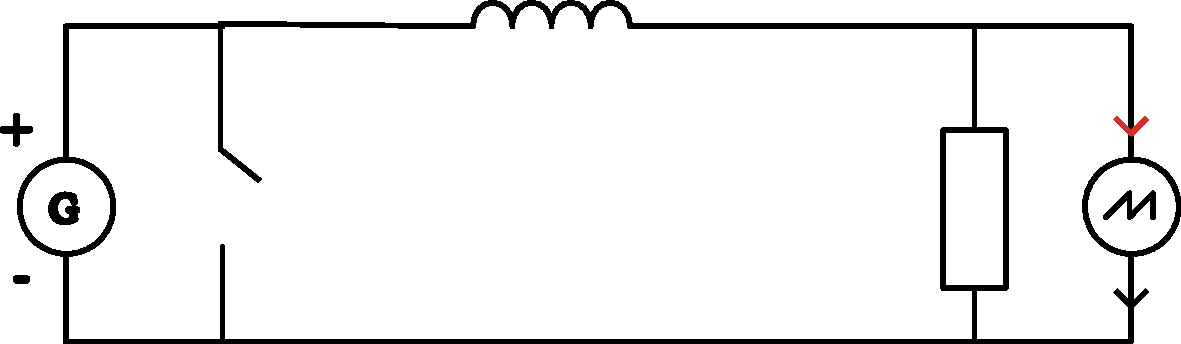
\includegraphics[scale=0.4]{s3}
 \end{center}
\caption{Montage expérimental}
\end{figure}

On réalise ce circuit avec $E = 3 \text{ V}$, $R = 10 \Omega$, et la bobine ($r_L \approx 9.5 \Omega$).
    



\subsection{Mesures à effectuer}
\subsubsection{Lois de faraday}
\begin{enumerate}
    \item Lancer une acquisition de 24s avec 2400 points et relever la valeur moyenne pour obtenir l'offsset de la carte avec Mesures Automatiques > Valeur Moyenne
    \item Après avoir lancé une nouvelle acquisuation 
\begin{itemize}
    \item Rentrer lentement la bobine C 1 vers la bobine F
    \item Répéter l'opération avec une vitesse moyenne
    \item Répéter l'opération avec une vitesse rapide
    \item Refaire les étapes précédentes en retournant la bobine
\end{itemize}
\end{enumerate}
\subsubsection{Inductance mutuelle}
On fait varier la fréquence de 2.0 kH à 20.0 kH par pas de 2.0 kH et on relève à l'aide l'oscilloscope les valeurs de $\Delta U$ et $E_2$.
   \subsubsection{Mesure du coefficient d'auto-induction}
   On règle d'abord Latis Pro.
    \begin{itemize}
        \item \textbf{Temps total ($T_{tot}$) :} Pour une bobine de $36 \text{ mH}$ et $R_{tot} \approx 16 \Omega$, $\tau \approx 2,2 \text{ ms}$. Il faut un temps total d'environ $5\tau \approx 12 \text{ ms}$ pour voir la décharge complète. On réglera $T_{tot} \approx 20 \text{ ms}$.
        \item \textbf{Échantillonnage :} Pour définir correctement l'exponentielle, il faut au moins 500 à 1000 points.
        \item \textbf{Déclenchement (Trigger) :} Voie EA1, sens descendant (puisqu'on observe la décharge), niveau de seuil à environ $2 \text{ V}$ pour une tension E de 3V environ et de 6V pour une tension originale de 12V environ. On ajoute de un près-trig de 25\%.
    \end{itemize}
    Il n'y a plus qu'a créer le court-circuit avec l'interrupteur et lancer l'acquisition.
\section{Mesures}
\subsection{Lois de faraday}
\subsubsection{Données}
Nous n'avons pas pu exporter les données brutes de Latis Pro. Nous fournissons les données traitées :

\begin{center}
\begin{tabular}{|c|c|c|}
\hline
\textbf{Mesure} & \textbf{Opération} & \textbf{Flux $\Phi$ (mWb)} \\
\hline
$\phi_1$ & Introduction 1 & $73,75$ \\
$\phi_2$ & Introduction 2 & $72,54$ \\
$\phi_3$ & Introduction 3 & $72,13$ \\
\hline
$\phi_4$ & Bobine retournée - Intro 1 & $-70,81$ \\
$\phi_5$ & Bobine retournée - Intro 2 & $-68,49$ \\
$\phi_6$ & Bobine retournée - Intro 3 & $-79,98$ \\
\hline
\end{tabular}
\end{center}
\subsubsection{Incertitudes}
%L'incertitude sur $\Phi$ provient principalement de la dérive résiduelle après soustraction de l'offset et du bruit de mesure (visible sur la courbe bleue). On estime l'incertitude expérimentale à environ $\pm 5\%$, soit $\Delta\Phi \approx 4 \text{ mWb}$.
L'incertitude sur le flux $\Phi$ est dominée par la dérive temporelle observée. Bien que normalement corrigée par l'offset de $7,1187 \text{ mV}$, une instabilité résiduelle $\delta V \approx 0,2 \text{ mV}$ sur 24 s génère une erreur cumulative. 

En appliquant une évaluation de type A sur les trois premières mesures :
\begin{itemize}
    \item Moyenne : $\bar{\Phi} = 72,81 \text{ mWb}$
    \item Écart-type : $s_{\Phi} = 0,84 \text{ mWb}$
    \item Incertitude élargie ($k=2$) : $\Delta \Phi \approx 2 \text{ mWb}$
\end{itemize}
Toutefois, compte tenu du bruit de fond et de la précision de la carte d'acquisition, nous retiendrons une incertitude de $\Delta\Phi = 5 \text{ mWb}$, couvrant l'ensemble des sources d'erreurs systématiques.
\subsection{Inductance mutuelle}
\subsubsection{Données}
Le tableau suivant présente les valeurs de fréquence $f$, de tension au primaire $\Delta U$ et de f.e.m. induite $E_2$. Nous calculons également la dérivée du courant $\frac{di_1}{dt} = \frac{2f \Delta U}{R}$.

\begin{center}
\begin{tabular}{|c|c|c|c|}
\hline
$f$ (Hz) & $\Delta U$ (V) & $E_2$ (V) & $\frac{di_1}{dt}$ (A/s) \\
\hline
2000  & 7,925 & 0,0440 & 158,5 \\
4000  & 7,916 & 0,0840 & 316,6 \\
6000  & 7,900 & 0,1255 & 474,0 \\
8000  & 7,850 & 0,1650 & 628,0 \\
10000 & 7,850 & 0,2090 & 785,0 \\
12000 & 7,830 & 0,2530 & 939,6 \\
14000 & 7,821 & 0,2950 & 1094,9 \\
16000 & 7,820 & 0,3375 & 1251,2 \\
18000 & 7,820 & 0,3795 & 1407,6 \\
20000 & 7,780 & 0,4220 & 1556,0 \\
\hline
\end{tabular}
\end{center}
De plus, la valeur de la résistance utilisée a été relevée à $199\Omega$.
\subsubsection{Incertitudes}
Comme précédemment, nous nous concentrons sur l'erreur de quantification de la carte d'acquisition pour $E_2$ (calibre $\pm 1$ V, 12 bits) :
$$u(E_2) = \frac{q}{\sqrt{12}} = \frac{2 / 2^{12}}{\sqrt{12}} \approx 0,14 \text{ mV}$$

Pour la régression linéaire $E_2 = M \cdot X$ (avec $X = \frac{di_1}{dt}$), l'incertitude sur la pente $M$ est estimée à partir de la dispersion des points expérimentaux (écart-type de la pente). Étant donné la précision des mesures de fréquence et de résistance, l'incertitude sur $X$ est négligée devant celle sur $E_2$.
\subsection{Mesure du coefficient d'auto-induction}
\begin{itemize}
    \item \textbf{Résistance totale du circuit :} $R_{tot} = R + r_L = 19,5 \, \Omega$.
    \item \textbf{Temps caractéristique mesuré ($\tau$) :} À l'aide de l'outil de modélisation (fit exponentiel $y = A \cdot e^{-x/B} + C$), nous avons identifié le paramètre $B = \tau$. La valeur obtenue est :
    $$\tau_{exp} = 0,00207 \text{ s} = 2,07 \text{ ms}$$
   \end{itemize}
\section{Graphiques}
\subsection{Lois de faraday}
La capture d'écran montre en bleu la tension $e(t)$ et en rose son intégrale (le flux).
\begin{figure}[H]
 \begin{center}
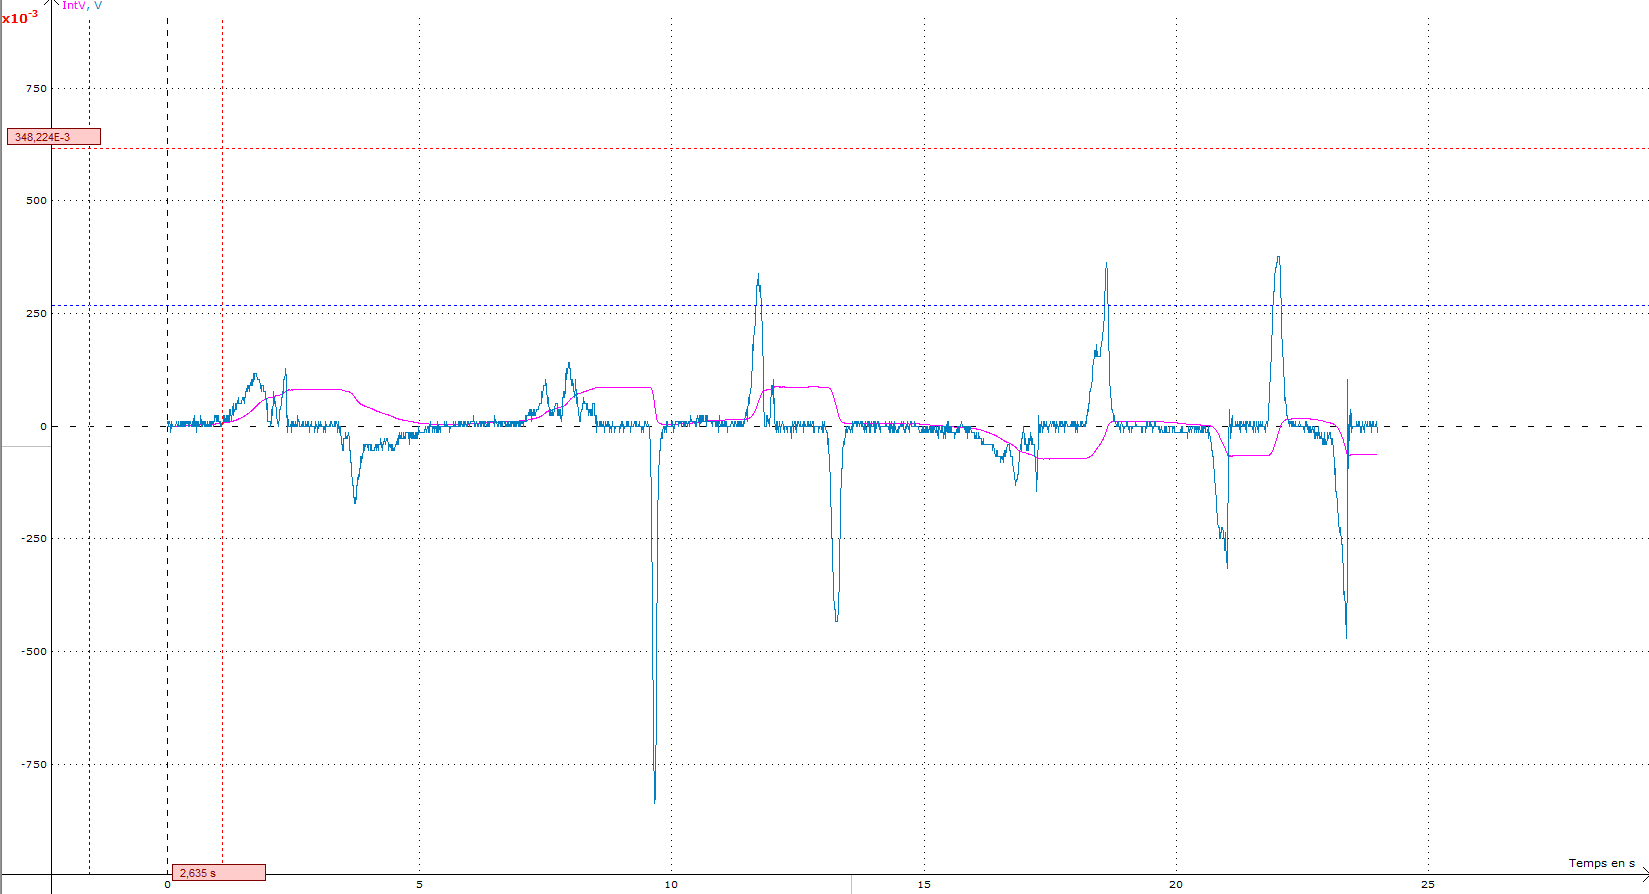
\includegraphics[scale=0.3]{fig_p1}
 \end{center}
\caption{Évolution de U (V) en fonction du temps (s)}
\end{figure}
\begin{itemize}
    \item Les pics de tension correspondent aux phases de mouvement.
    \item L'amplitude du pic dépend de la vitesse, mais l'aire sous la courbe (le flux final) reste constante.
    \item Le palier de flux en rose indique que la bobine est immobile à l'intérieur du champ.
\end{itemize}
\subsection{Inductance mutuelle}
\begin{figure}[H]
 \begin{center}
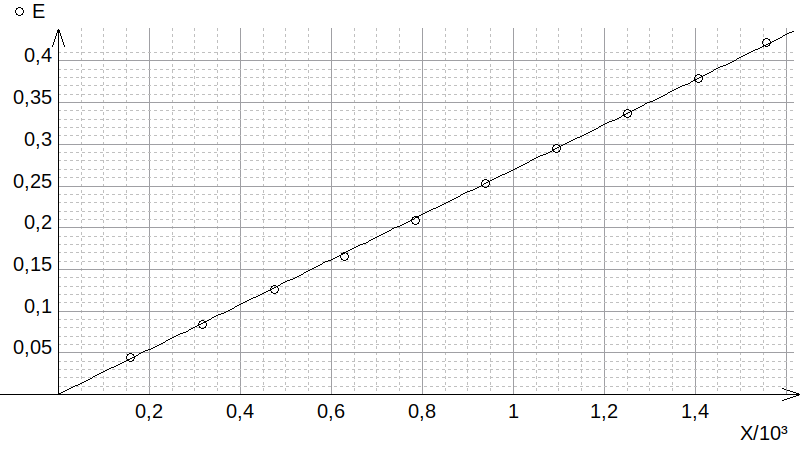
\includegraphics[scale=0.4]{fig_p2}
 \end{center}
\caption{Évolution de E (V) en fonction de  $X = \frac{\dd i_1}{\dd t}$}
\end{figure}
\subsection{Mesure du coefficient d'auto-induction}
\begin{figure}[H]
 \begin{center}
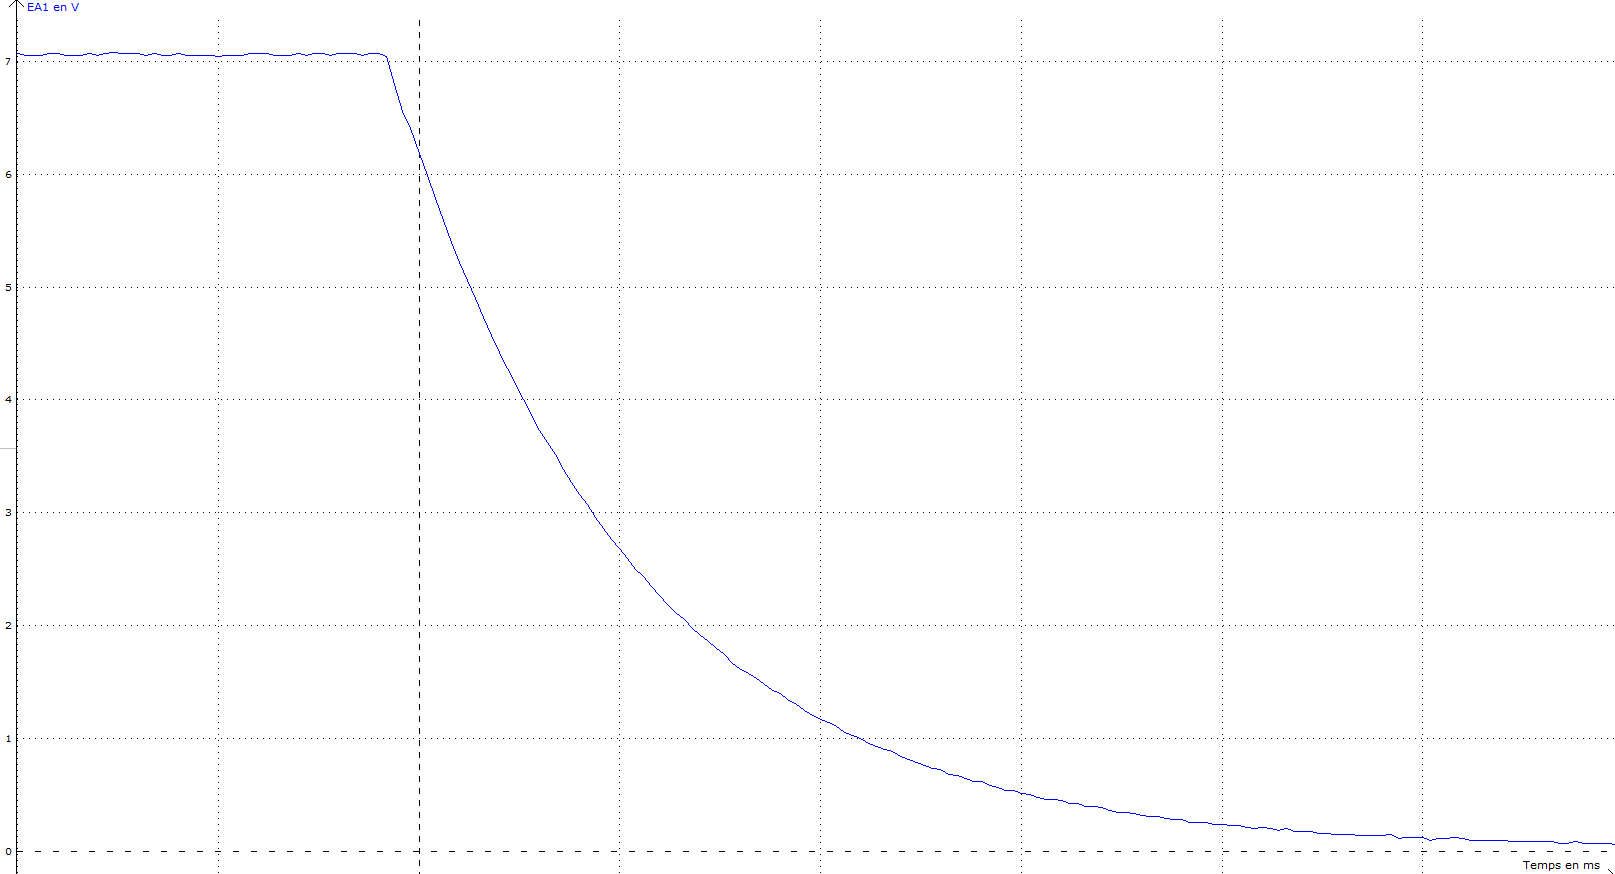
\includegraphics[scale=0.3]{fig_p3}
 \end{center}
\caption{Évolution de la tension (V) en fonction du temps (ms)}
\end{figure}

\section{Exploitation des résultats}
\subsection{Lois de faraday}
\subsubsection{Analyse Qualitative (Faraday-Lenz)}
1. \textbf{Mouvement :} Lorsqu'on déplace l'aimant, l'aiguille du galvanomètre dévie, indiquant un courant. Si la vitesse augmente, la déviation est plus grande ($|e| \propto |d\Phi/dt|$). \\
2. \textbf{Loi de Lenz :} En approchant le pôle Nord, le flux augmente. Le courant induit crée un champ magnétique opposé (pôle Nord face à l'aimant), créant une force répulsive. C'est l'affirmation 2 qui est vraie : \textit{"Le champ magnétique induit s'oppose à la variation du champ magnétique de l'aimant."} \\
3. \textbf{Circuit ouvert :} Avec un voltmètre (haute impédance), le courant est quasi nul, donc pas de champ induit significatif, mais une tension $e$ est bien présente.

\subsubsection{Analyse Quantitative (Flux)}
\textbf{Effet de la vitesse :} On observe sur le graphique que pour $\phi_1, \phi_2, \phi_3$, malgré des vitesses d'introduction différentes (pics de hauteurs variées), le flux final atteint est quasi identique ($\approx 72,8 \text{ mWb}$ en moyenne). Cela confirme que le flux $\Phi$ ne dépend que de la position géométrique finale de la bobine. \\
\textbf{Retournement de la bobine :} Le retournement change le sens de l'enroulement par rapport au champ $\vec{B}$. On observe un changement de signe ($\phi_4, \phi_5, \phi_6 \approx -73 \text{ mWb}$), ce qui est cohérent avec le produit scalaire $\Phi = \iint \vec{B} \cdot d\vec{S}$.
\subsection{Inductance mutuelle}

\subsubsection{Calcul du coefficient M}
On trace sur Regressi $E_2 = f(X) = a X$ avec $X = 2f\frac{\Delta U}{R}$ Le coeffcient $a$ sera alors de M recherchée.
En effectuant une régression linéaire sur les données du tableau, nous obtenons la pente $M$.

On obtient alors $M_{exp} = 2.60\cdot 10^{-4}$, pour $R = 199.8\Omega$.

\subsubsection{Comparaison avec la valeur attendue}
La valeur théorique pour deux solénoïdes imbriqués, en considérant le primaire comme un solénoïde long, est donnée par :
$$M_{th} = \mu_0 \frac{N_1 N_2}{l_1} S$$
Avec les nouvelles données géométriques :
\begin{itemize}
    \item Diamètre $D = 4,7 \text{ cm} \implies$ Rayon $r = 2,35 \text{ cm} = 0,0235 \text{ m}$
    \item Section $S = \pi \cdot r^2 = \pi \cdot (0,0235)^2 \approx 1,735 \cdot 10^{-3} \text{ m}^2$
    \item $N_1 = 200$, $N_2 = 200$, $l_1 = 0,4 \text{ m}$
\end{itemize}

Le calcul numérique donne alors :
$$M_{th} = 4\pi \cdot 10^{-7} \cdot \frac{200 \cdot 200}{0,4} \cdot 1,735 \cdot 10^{-3} \approx 0,218 \cdot 10^{-3} \text{ H} = \mathbf{0,218 \text{ mH}}$$

\subsubsection{Analyse des écarts}
Nous obtenons maintenant une valeur théorique $M_{th} = 0,218 \text{ mH}$ pour une valeur expérimentale $M_{exp} \approx 0,269 \text{ mH}$. 

L'écart relatif est de :
$$\epsilon = \frac{|M_{exp} - M_{th}|}{M_{th}} \approx 23\%$$

Plusieurs facteurs expliquent que la valeur expérimentale soit légèrement supérieure à la théorie simplifiée du solénoïde long :
\begin{itemize}
    \item \textbf{Épaisseur du bobinage :} Le rayon effectif est souvent légèrement supérieur au rayon intérieur $r$ à cause de l'épaisseur des couches de fils, ce qui augmente la section $S$ réelle.
    \item \textbf{Erreur sur la longueur $l_1$ :} Si les spires ne sont pas parfaitement jointives ou si la longueur bobinée est plus courte que 40 cm, $M$ augmente.
    \end{itemize}

L'ordre de grandeur est cependant parfaitement validé, confirmant la bonne compréhension du phénomène d'induction mutuelle.
\subsection{Mesure du coefficient d'auto-induction}
\subsubsection{Établissement des formules}
Lorsqu'on ferme l'interrupteur, la maille (générateur déconnecté) donne :
$$L\frac{di}{dt} + (R + r_L)i = 0 \implies \frac{di}{dt} + \frac{R_{tot}}{L}i = 0$$
La solution est une décroissance exponentielle : $i(t) = I_0 e^{-t/\tau}$ avec $\tau = \frac{L}{R+r_L}$.
La tension mesurée aux bornes de la résistance est alors : $u_R(t) = R \cdot I_0 e^{-t/\tau}$.

\subsubsection{Modélisation}


En utilisant la relation théorique $\tau = \frac{L}{R_{tot}}$, nous en déduisons la valeur expérimentale de l'inductance propre de la bobine :
    $$L_{exp} = \tau_{exp} \cdot R_{tot} = 0,00207 \times 19,5$$
    $$\mathbf{L_{exp} \approx 0,0404 \text{ H} \approx 40,4 \text{ mH}}$$

\subsubsection{Incertitudes}
L'incertitude sur $L$ est calculée par propagation d'incertitude sur le produit $L = \tau \cdot R_{tot}$. 

N'ayant pas mesuré les valeurs réelles des résistances au multimètre, nous devons nous fier aux données constructeur. Nous estimons une incertitude élargie de \textbf{5\%} sur $R$ (résistance de précision standard) et de \textbf{10\%} sur la résistance interne de la bobine $r_L$ (souvent sujette à des variations d'échauffement ou de fabrication). 

L'incertitude relative sur $R_{tot}$ est alors estimée à :
$$\frac{u(R_{tot})}{R_{tot}} \approx 7\%$$

En combinant cela avec l'incertitude du fit sur $\tau$ (estimée à $2\%$), l'incertitude relative sur $L$ devient :
$$\frac{u(L)}{L} = \sqrt{(2\%)^2 + (7\%)^2} \approx 7,3\%$$

L'incertitude absolue est donc $\Delta L = 40,4 \times 0,073 \approx 3 \text{ mH}$.
On retiendra finalement : $\mathbf{L = 40 \pm 3 \text{ mH}}$.


\subsubsection{Comparaison avec la valeur théorique}
La valeur nominale constructeur est $L_{th} = 36 \text{ mH}$. 
L'écart relatif est de $$\epsilon = \frac{|L_{exp} - L_{th}|}{L_{th}} =12,2\%$$. 

\subsubsection{Analyse de la fiabilité des résultats}
L'écart entre la valeur expérimentale ($40 \text{ mH}$) et la valeur théorique ($36 \text{ mH}$) doit être interprété avec précaution pour deux raisons majeures liées à l'absence de mesures directes :

\begin{itemize}
    \item \textbf{Incertitude sur les résistances :} Comme nous n'avons pas vérifié $r_L$ et $R$ au multimètre, une partie de l'erreur sur $L$ provient probablement d'une sous-estimation de la résistance totale dans notre calcul. Si $R_{tot}$ réel était légèrement plus faible, $L$ se rapprocherait de $36 \text{ mH}$.
    \item \textbf{Impédance du générateur :} Nous avons négligé la résistance interne du générateur ($R_g$). Si celle-ci n'est pas nulle, elle s'ajoute à $R_{tot}$, ce qui augmenterait encore la valeur calculée de $L$.
\end{itemize}

Cependant, comme $L_{th}$ ($36 \text{ mH}$) se rapproche très fortement de l'intervalle d'incertitude élargi $[37 ; 43] \text{ mH}$, on peut conclure que la manipulation est cohérente avec le modèle théorique.



\section{Conclusion}
%\textit{Récapitulatif des valeurs trouvées, comparaison avec les données constructeur et validation de la loi de Faraday-Lenz.}
% \newpage
% WIP

% \section{Mesure du coefficient d'auto-induction L}

% \subsection{Objectifs}
% L'objectif est de mesurer l'inductance propre $L$ d'une bobine en étudiant la réponse transitoire d'un circuit $RL$ lors de la décharge de l'énergie emmagasinée. Nous comparerons la valeur expérimentale à la valeur théorique constructeur ($36 \text{ mH}$).

% \subsection{Réponses aux questions théoriques}
% \subsubsection{Ordre des composants}
% \textbf{Question : Peut-on mettre la bobine et la résistance dans n'importe quel ordre ?} \\
% En théorie (loi des mailles), l'ordre n'affecte pas le comportement global du circuit. Cependant, pour la mesure à l'oscilloscope ou via la carte d'acquisition, il est impératif que l'un des composants soit relié à la \textbf{masse commune}. Comme on souhaite observer le courant $i(t)$ à travers la tension $u_R(t) = R \cdot i(t)$, on place généralement la résistance côté masse.

% \subsubsection{Établissement des formules}
% Lorsqu'on ferme l'interrupteur, la maille (générateur déconnecté) donne :
% $$L\frac{di}{dt} + (R + r_L)i = 0 \implies \frac{di}{dt} + \frac{R_{tot}}{L}i = 0$$
% La solution est une décroissance exponentielle : $i(t) = I_0 e^{-t/\tau}$ avec $\tau = \frac{L}{R+r_L}$.
% La tension mesurée aux bornes de la résistance est alors : $u_R(t) = R \cdot I_0 e^{-t/\tau}$.

% \subsection{Protocole et Réglages}
% \begin{itemize}
%     \item \textbf{Montage :} Circuit série avec $E = 3 \text{ V}$, $R = 10 \Omega$, et la bobine ($r_L \approx 6 \Omega$).
%     \item \textbf{Réglages Latis Pro :}
%     \begin{itemize}
%         \item \textbf{Temps total ($T_{tot}$) :} Pour une bobine de $36 \text{ mH}$ et $R_{tot} \approx 16 \Omega$, $\tau \approx 2,2 \text{ ms}$. Il faut un temps total d'environ $5\tau \approx 12 \text{ ms}$ pour voir la décharge complète. On réglera $T_{tot} \approx 20 \text{ ms}$.
%         \item \textbf{Échantillonnage :} Pour définir correctement l'exponentielle, il faut au moins 500 à 1000 points.
%         \item \textbf{Déclenchement (Trigger) :} Voie EA1, sens descendant (puisqu'on observe la décharge), niveau de seuil à environ $2 \text{ V}$.
%     \end{itemize}
% \end{itemize}


% \section{Exploitation des résultats}

% \subsection{Détermination de L}
% Après acquisition, nous utilisons la fonction d'ajustement $y = A \cdot \exp(-x/B) + C$ de Latis Pro ou Regressi.
% \begin{itemize}
%     \item Le paramètre $B$ correspond au temps caractéristique $\tau$.
%     \item Nous en déduirons $L = \tau \cdot (R + r_L + R_g)$.
% \end{itemize}

% \subsection{Analyse critique}
% La résistance interne de la bobine $r_L$ doit être mesurée à l'ohmmètre pour ne pas fausser le calcul de $L$. Si la valeur obtenue s'éloigne des $36 \text{ mH}$, nous vérifierons si le noyau de fer (entrefer) était présent ou non, car sa perméabilité $\mu_r$ augmente drastiquement la valeur de $L$.


Ce TP a permis de valider les lois fondamentales de l'électromagnétisme à travers trois approches complémentaires :

\begin{itemize}
    \item \textbf{Loi de Faraday-Lenz :} L'étude qualitative a confirmé le caractère modérateur du courant induit. L'approche quantitative a démontré que le flux magnétique ($\Phi \approx 73$~mWb) est une fonction d'état indépendante de la vitesse de balayage.
    \item \textbf{Inductance mutuelle :} La mesure de $M$ en régime sinusoïdal ($\approx 0,27$~mH) confirme l'ordre de grandeur théorique, malgré un écart de 23\% imputable aux limites du modèle du solénoïde infini et aux fuites de flux.
    \item \textbf{Auto-induction :} L'étude du régime transitoire a permis de mesurer $L = 40 \pm 3$~mH. L'écart de 12\% avec la valeur constructeur (36~mH) reste cohérent compte tenu des incertitudes sur les résistances internes ($r_L$ et $R_g$).
\end{itemize}

\begin{center}
\begin{tabular}{|l|c|c|c|}
\hline
\textbf{Grandeur} & \textbf{Valeur Exp.} & \textbf{Valeur Th./Ref.} & \textbf{Écart relatif} \\ \hline
Flux $\Phi$ & 72,8 mWb & - & - \\ \hline
Mutuelle $M$ & 0,27 mH & 0,22 mH & 23 \% \\ \hline
Inductance $L$ & 40,4 mH & 36,0 mH & 12 \% \\ \hline
\end{tabular}
\end{center}

En conclusion, malgré les limites de précision des composants et de la chaîne d'acquisition, les phénomènes d'induction ont été caractérisés avec une précision satisfaisante.
\end{document}